% \textbf{Title: ImpulseAndMomentum 1}

Two identical bullets are fired horizontally with identical speeds $v_0$ at two blocks of equal mass. The blocks rest on a frictionless horizontal surface and are made of hard steel and soft wood respectively, see figure. One bullet bounces elasticcally off the steel block. The other bullet becomes embedded inside the wood block.
Which one of the following statements best describes which block travels faster after the collision?

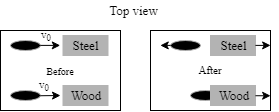
\includegraphics[width=3in]{../../Images/ImpulseAndMomentumQ1.png}\\

a. The wood block, because it has gained the momentum of the bullet, while the other bullet does not impart its momentum to the seel block.

b. The wood block, because it transfers all of its kinetic energy to it.

*c. The steel block, because the bullet bounces off from it.

d. Both blocks travel with the same speed.

e. I do not know.\\
